\section{Zielsetzung}

\noindent In diesem Versuch wird eine Methode zur Bestimmung der Halbwertszeit $T$ unterschiedlicher Atome durch Aktivierung mittels Neutronen untersucht.

\section{Theorie}

\subsection{Kernreaktionen mit Neutronen}

\noindent Kernreaktionen sind im allgemeinen Reaktionen eines Teilchens mit dem Kern eines Atoms. In diesem Verusch werden die Wechselwirkungen 
von Neutronen mit einem Kern genauer untersucht. Absorbiert ein Kern A ein Neutronen bei solch einer Wechselwirkungen entsteht ein neuer Kern
$\text{A}^{\ast}$, dieser wird Zwischenkern oder Compound Kern genannt. Der Kern $\text{A}^{\ast}$ nimmt die kinetische und die Bindungsenergie 
des Neutrons auf und liegt somit energetisch über dem Kern A. Diese Energie wird dann innerhalb des Kerns auf die einzelnen Nukleonen verteilt, 
somit reicht die Energie nicht mehr aus um ein Nukleon des Kerns wieder auszustoßen. Um nun wieder in den Grundzustand zurück zu kommen gibt der 
angeregter Kern Energie in Form eines $\upgamma$-Quants nach etwa $\SI{10e-16}{\second}$ ab.\\
Es läuft folgende Reaktion ab:

\begin{equation*}
   \ce{^m_z\symup{A} + ^1_0\symup{n} -> ^{m+1}_z\symup{A}^{\ast} -> ^{m+1}_z \symup{A} + \upgamma }. \nonumber
\end{equation*}

\noindent Mit der Massenzahl m des Kern. Der hier entstandene Kern $\ce{^{m+1}_z \text{A}}$ ist meistens instabil, da er ein Neutron mehr hat als ein 
stabiler Kern gleicher Ordnungszahl. Aufgrund des emissierten $\gamma$-Quants ist der Kern jedoch nicht angeregt und somit relativ langlebig.
Durch Emission eines Elektrons wird der Kern wieder stabil.

\begin{equation*}
   \ce{^{m+1}_z \symup{A} -> ^{m+1}_{z+1} \symup{C} + \upbeta^- + \symup{E_{kin}} + \bar{\symup{\nu}}_{\symup{e}}} \nonumber
\end{equation*}

\noindent $\bar{\symup{\nu}}_{\symup{e}}$ ist hier ein Antineutrino. Dieses Antineutrino ensteht da die Masse des Kerns $\ce{^{m+1}_z \text{A}}$ 
größer als Massen der rechten Seite ist. Die restliche Masse ist nach der Beziehung

\begin{equation*}
   \Delta E = \Delta m c^2 \nonumber
\end{equation*}

\noindent in kinetische Energie von Elektron und Antineutrino umgewandelt.\\
Die Wahrscheinlichkeit, dass ein Kern ein Neutron einfängt wird als Wirkungsquerschnitt $\sigma$ bezeichnet. Dieser gibt ein Verhältnis der 
Einfangwahrscheinlichkeit in Abhängigkeit von gewissen Material Eigenschaften an und hat somit die Einheit einer Fläche.

\begin{equation*}
   \sigma = \frac{u}{nKd} \nonumber
\end{equation*}

\noindent Mit $u$ der Einfänge, $n$ der Neutronen pro Sekunde, $d$ der Dicke und $K$ der Atomdichte der Folie. $\sigma$ wird angepasst an den 
Kernquerschnitt in $\si{\barn} \coloneqq \SI{10e-24}{\centi\metre\squared}$ angegeben. Da der Wirkungsquerschnitt stark von der kinetischen Energie 
der einfallenden Teilchen abhängt, wird hier zwischen schnellen und langsamen Neutronen unterschieden. Die Wellenlänge eines Neutrons 
berechnet sich mittels der De-Broglie-Wellenlänge:

\begin{equation*}
   \lambda = \frac{h}{m_{\symup{n}}v}. \nonumber
\end{equation*}

\noindent Hier ist $h$ das Planksche Wirkungsquantum, $m_n$ die Neutronenmasse und $v$ die Geschwindigkeit des Neutrons. Für große Geschwindigkeiten 
und somit kleine Wellenlänge im Verhältnis zum Kernradius R($\approx \SI{10e-12}{\centi\meter}$), lassen sich geometrische Überlegungen auf die 
wechselwirkungs Wahrscheinlichkeit anwenden. Es besteht eine Analogie zur optischen Streuung von Wellen and Verhältnismäßig großen Objekten. ­Für 
große Wellenlängen entstehen wieder wie in der Analogie zur Optik, Interferenzeffekte, somit sind geometrische Überlegungen unbrauchbar. Das 
Experiment zeigt eine Neutronengeschwindigkeit bei der, der Wirkungsquerschnitt deutliche größer als der geometrische Querschnitt. Dieser Effekt
entsteht, wenn die Neutronenenergie gleich der Differenz zweier Energienevaus im Zwischenkern. Die durch Breit und Wigner angegebene Formel:

\begin{equation*}
   \sigma(E) = \sigma_0 \sqrt{ \frac{E_{\symup{r_i}}}{E} } \frac{\tilde{c}}{\left( E - E_{\symup{r_i}} \right)^2 + \tilde{c}} \nonumber
\end{equation*}

\noindent beschreibt den Wirkungsquerschnitt in Abhängigkeit der Neutrönenergie $E$. Hier sind $\tilde{c}$ und $\sigma_0$ charakterische 
Konstanten und $E_{\symup{r_i}}$ die Energienevaus. Aus der Formel ist abzulesen, dass $\sigma$ für $E$=$ E_{\symup{r_i}}$ maximal wird.
Ist $E$ jedoch deutlich kleiner als $E_{\symup{r_i}}$, kann $\left( E - E_{\symup{r_i}} \right)^2$ als Konstante angenommen werden. Dadurch ist:

\begin{equation*}
   \sigma \sim \frac{1}{\sqrt{E}} \sim \frac{1}{v} . \nonumber
\end{equation*}

\noindent Diese Antiproportionalität von $\sigma$ und $v$ deckt sich mit der Vorstellung, dass bei kleineren Geschwindigkeiten, das Neutron mehr 
Zeit hat um mit dem Kern zu wechselwirken.

\subsection{Erzeugung niederenergetischer Neutronen}

\noindent Da die beschriebenen niederenergetischen Neutronen in der Natur aufgrund ihrer Instabilität nicht vorkommen, müssen sie zunächst in einer 
Kernreaktion freigesetzt werden. Dies geschiet in diesem Versuch durch den Beschuss von $\ce{^9\symup{Be}}$-Kernen mit \alpha-Teilchen:

\begin{equation*}
   \ce{ ^9_4 \symup{Be} + ^4_2$\alpha$ -> ^{12}_6\symup{C} + ^1_0\symup{n}} .\nonumber
\end{equation*}

\noindent Die \alpha-Teilchen entstehen bei dem Zerfall von $\ce{^{226} \text{Ra}}$-Kernen. Die bei der Wechselwirkung mit den 
$\ce{^9\symup{Be}}$-Kernen frei werdenden Neutronen haben aber noch zu viel Energie und müssen abgebremst werden. Dies geht nach der Formel für 
elastische Stöße:

\begin{equation*}
   E_{\symup{ü}}  = E_0 \frac{4Mn}{\left( M + m \right)^2} \nonumber
\end{equation*}

\noindent am besten wenn die Massen der Stoßpartner möglichst gleich sind. Somit ist der optimale Stoßpartner Wasserstoff. Die Neutronenquelle wird 
deshalb von einem Mantel aus Paraffin $\left( \symup{C_n H_{2n+2}} \right)$ umgeben (siehe Abb \ref{img:Paraffin}).

\begin{figure}[H]
   \centering
   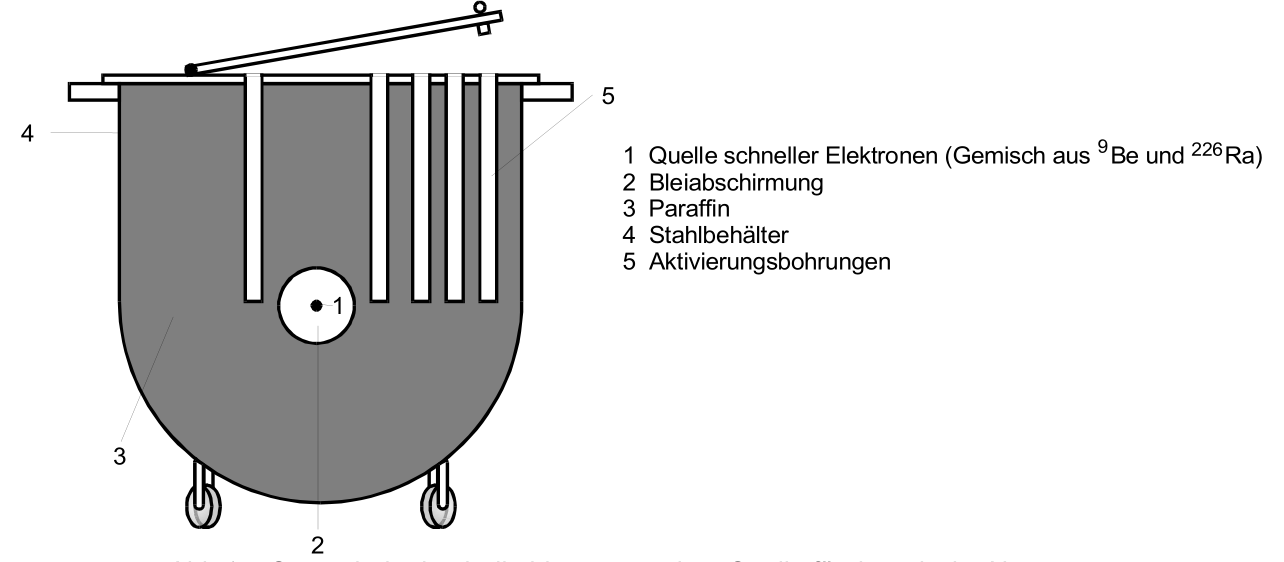
\includegraphics[width=0.75\textwidth]{images/Theorie1.PNG}
   \caption{Querschnitt durch die hier verwendete Quelle für thermische Neutronen \protect \cite{V702}.}
   \label{img:Paraffin}
\end{figure}

\noindent Die Neutronen haben nun bevor sie bei den zu aktivierenden Kernen ankommen die mittlere kinetische Energie des Paraffins. Dies entspricht 
bei 290 Kelvin in etwas 0,025 eV. Die Neutronen mit dieser Energie werden als thermische Neutronen bezeichnet. 

\subsection{Untersuchung des Zerfalls instabiler Isotope}

\noindent Beispiele von Isotopen die durch Wechselwirkungen mit Neutronen instabil werden, sind folgende:

\begin{equation*}
   \ce{^{51} \symup{V}, ^{55}\text{Mn}, ^{79}\text{Br}, ^{115}\text{In}, ^{127}\text{J}, ^{164}\text{Dy}, ^{107}{Ag}, ^{109}\text{Ag}, ^{103}\text{Rh}} \nonumber
\end{equation*}

\noindent Die Halbwertszeiten der $\upbeta ^-$-Zerfälle der instabilen Isotope liegen zwischen Sekunden und Stunden. Die Aktivierung und der 
Zerfall von Ag und Rh verläuft gemäß der folgenden Reaktionsgleichungen:

\begin{equation}
   \ce{^{107}_{47}\text{Ag} + \symup{n} -> ^{108}_{47}\text{Ag} -> ^{108}_{48}\text{48} + $\upbeta$^- + \bar{\symup{\nu}}_{\symup{e}}} 
   \label{eq:Ag107}
\end{equation}

\begin{equation}
   \ce{^{109}_{47}\text{Ag} + \symup{n} -> ^{110}_{47}\text{Ag} -> ^{110}_{48}\text{48} + $\upbeta$^- + \bar{\symup{\nu}}_{\symup{e}}}
    \label{eq:Ag109} 
\end{equation}

\begin{equation}
   \begin{split}
      \ce{^{103}_{45}\text{Rh} + \symup{n}} \mathbin{\scalebox{2.5} \textbraceleft } \quad
   \end{split}
   \begin{split}
      &\overset{10\%}{\longrightarrow} \ce{^{104\symup{i}}_{45}\text{Rh} -> ^{104}_{45}\text{Rh} + $\upgamma$ -> ^{104}_{46}\text{Pd} + $\upbeta$^- + \bar{\symup{\nu}}_{\symup{e}} } \\
      &\overset{90\%}{\longrightarrow} \ce{^{104}_{45}\text{Rh} -> ^{104}_{46}\text{Pd} + $\upbeta$^- +\bar{\symup{\nu}}_{\symup{e}} } \\
   \end{split}
   \label{eq:Rh103}
\end{equation}

Die Zerfälle der anderen Isotope verhalten sich nach dem gleichen Schema von $\ce{^{107}_{47}\text{Ag und}^{109}_{47}\text{Ag}}$.\\
Ziel ist es nun die Halbwertszeiten der Zerfälle zu bestimmen. Dazu wird das Zerfalls Gesetz:

\begin{equation}
   N(t) = N_0 \symup{e}^{- \lambda t} 
   \label{eq:4}
\end{equation}

\noindent benötigt. $N_0$ ist hier die Anzahl der zu Anfang vorhandenen Kerne und $\lambda$ die Zerfallskonstante. Die Zerfallskonstante gibt an 
wie wahrscheinlich es ist, dass ein Kern zerfällt. Somit besteht ein direkter Zusammenhang zwischen \lambda und der Halbwertszeit $T$.
Durch die Gleichung:

\begin{equation*}
   \frac{N_0}{2} = N_0 \symup{e}^{- \lambda T} 
\end{equation*}

\noindent ergibt sich folgender Zusammenhang:

\begin{equation*}
   T = \text{ln}\left(\frac{2}{\lambda}\right) . \nonumber
\end{equation*}

\noindent Im Grunde wäre es nun möglich mittels Gleichung\ref{eq:4} die Halbwertszeit zu bestimmen, jedoch ist es in der Praxis schwierig, 
zuverlässig $N(t)$ zu bestimmen. Es ist deutlich einfacher die frei werdende Strahlung bei den einzelnen Zerfällen zu messen.
Daher wird eine Definition für $N_{\Delta t}(t)$ eingeführt:

\begin{equation}
   N_{\Delta t}(t) = N(t) - N(t + \Delta t) . \nonumber
\end{equation}

\noindent Daraus folgt mittels Gleichung(\ref{eq:4}):

\begin{equation}
   N_{\Delta t}(t) = N_0 \symup{e}^{ - \lambda t} - N_0 \symup{e}^{- \lambda \left( t + \Delta t \right) } = N_0 \left( 1 - \symup{e}^{-\lambda \Delta t} \right) \symup{e}^{-\lambda t} \nonumber
\end{equation}

\noindent und

\begin{equation}
   \text{ln} \left( N_{\Delta t}(t)\right) = \text{ln} \left( N_0 \left( 1- \symup{e}^{-\lambda \Delta t}\right) -\lambda t \right) .
\label{eq:5}
\end{equation}

\noindent Aus der Gleichung ist zu erkennen, dass \lambda durch eine Ausgleichsgerade bestimmt werden kann, da 

\begin{equation}
   \text{ln}\left(N_0\left(1- \symup{e}^{-\lambda\Delta t}\right)  \right) \nonumber
\end{equation}

\noindent konstant ist. Das Problem bei dieser Methode ist es, das richte $\Delta t$ zu wählen, da ein zu kleines $\Delta t$ zu statistischen und 
ein zu großes $\Delta t$ zu systematischen Fehlern führt.

\subsubsection{Silber}

\noindent Silber stellt ein problem an dieses Verafahren da natürliches Silber zu 52,3 \% aus $\ce{^{107}\text{Ag}}$ und zu 48,7\% aus $\ce{^{109}\text{Ag}}$ 
besteht. Somit laufen zwei Zerfallsprozesse gleichzeitig ab sobald das Silber aktiviert wird. Jedoch zerfällt $\ce{^{110}\text{Ag}}$ deutich schneller 
als $\ce{^{108}\text{Ag}}$. Somit ist es möglich erst den Zerfall des langlebigen Isotop zu charakterisieren, nachedem das kurzlebige Isotop so gut 
wie komplett zerfallen ist. Dann werden die Anschläge die auf das langlebige Isotop zurück zu führen sind, von den gesamt Anschlägen abgezogen. Mit 
den Daten ist es dann möglich auch für das kurzlebige Isotop eine Ausgleichsgerade aufzustellen und die Halbwertszeit zu bestimmen.

\subsubsection{Rhodium}

\noindent Beim aktivieren des Rhodiums entsteht nur zu 90\% $\ce{^{104}\text{Rh}}$, die restlichen 10\% werden wie in \ref{eq:Rhodium} zu sehen
zu $\ce{^{104i}\text{Rh}}$, dieses geht dann durch Emission eine $\gamma$-Quants auch in ein $\ce{^{104}\text{Rh}}$ Kern über. Diese Prozesse 
laufen Zeitgleich mit unterschiedlichen Halbwertszeiten ab, jedoch kann die \gamma-Strahlung seperat detektiert werden und dann wie beim Silber 
getrennt werden. 



%\begin{equation}
%   N_{\Delta t_{l}} \coloneqq N_{0_l}\left( 1- \symup{e}^{-\lambda_{l} \Delta t}\right) \symup{e}^{\lambda_l t} \nonumber
%\end{equation}
%
%
%\begin{equation}
%   N_{\Delta t} (t_{\symup{i}}) = N_{\Delta t , \text{gem}}(t_{\symup{i}}) - N_{\Delta t, \symup{u}} \nonumber
%\end{equation}